% This LaTex template is for manuscripts to be included in
% ISCA conference proceedings.
%
\documentclass[letterpaper,twocolumn]{article}
%
\usepackage[raggedright]{titlesec}
%
% include packages as needed, such as
\usepackage{amsmath}
\usepackage{amsthm}
\usepackage{graphicx}
\usepackage[ruled,vlined]{algorithm2e}
\usepackage{array}
\usepackage{multirow}
\usepackage{url}
%\usepackage{subfigure}
\usepackage[caption=false]{subfig}
\usepackage{romannum}
\usepackage{arydshln}
\hyphenation{op-tical net-works semi-conduc-tor}
\usepackage{subfloat}
\usepackage{amssymb}
\usepackage{multirow}
\usepackage[flushleft]{threeparttable}
\pagestyle{empty}

\setlength{\textwidth}{7.0in}
\setlength{\textheight}{9.125in}
\setlength{\columnsep}{0.375in}
\setlength{\topmargin}{-0.8in}
\setlength{\oddsidemargin}{-0.25in}
\setlength{\evensidemargin}{-0.25in}
\setlength{\parindent}{0.125in}
\setlength{\parskip}{1mm}

\renewcommand\labelenumi{(\theenumi)}

\date{}

\titlespacing{\section}{0pt}{*2.0}{*2.0}
\titlespacing{\subsection}{0pt}{*1.8}{*1.8}

\renewcommand{\topfraction}{0.9}
\renewcommand{\textfraction}{0.1}

\hyphenpenalty=5000
\tolerance=1000

\begin{document}

% Change to your title
\title{\Large\textbf{Clustering Metagenome Sequences Using Canopies}\normalsize}

%Chane authors, institutions and emails
\author {Mohammad Arifur Rahman, Nathan LaPierre, Huzefa Rangwala and Daniel Barbara\\
Department of Computer Science, George Mason University\\
Fairfax, VA, United States\\
mrahma23@gmu.edu, nlapier2@gmu.edu, rangwala@cs.gmu.edu, dbarbara@gmu.edu
}
\maketitle 
\thispagestyle{empty}
\begin{center}
\large\textbf{Abstract}
\end{center}
\vspace{2mm}
Advances in biotechnologies has allowed for the collective sequencing of co-existing microbial communities (Metagenomics). These microbial communities are ubiquitous across various clinical and ecological environments. Metagenomics has spurred the development of several bioinformatics approaches for analyzing the diversity, abundance and functions of different organisms within these communities.

We present a fast and scalable clustering algorithm for analyzing large-scale metagenome sequence data. Our approach achieves efficiency by partitioning the large number of sequence reads into groups (called canopies) using locality sensitive hashing. These canopies are then refined by using state-of-the-art sequence clustering algorithms. This two-phase approach allows for the use of our developed canopy-clustering algorithm as a pre-processing phase for computationally expensive clustering algorithms.

We evaluate our clustering algorithm on synthetic and real world 16S and whole metagenome  benchmarks. We demonstrate the ability of our proposed approach to  determine meaningful OTU assignments and observe significant speedup with regards to run time when compared to three different clustering algorithms. We also make our source code publicly available on Github\footnote{https://github.com/mrahma23/LSH-Canopy}. 

\medskip
\noindent
\textbf{keywords:} Clustering, Canopy, Metagenome, 16S, Biodiversity 

\section{Introduction} 
A large portion of the  earth's biomass 
comprises trillions of tiny  microorganisms 
with varying  biodiversity.  Communities
of interacting microbes  exists in several 
ecosystems ranging from the soil, ocean 
and human body\cite{MARHumanMicro}. Though, most of 
these microbes 
are beneficial to the host some are known to cause 
unwanted conditions and can be linked to cause of 
diseases in the host. 

\emph{Metagenomics} is the 
sequencing of the collective DNA  of 
microbial organisms coexisting as communities. Analyzing 
metagenomes has provided an unprecedented 
opportunity to understand the diversity, role and 
function of these organisms within different 
clinical and ecological environments\cite{MARHumanGut}\cite{MARMihaiPop}.

However, sequencing technologies do not deliver the 
complete genome of an organism (millions in length), but 
large number of short contiguous 
subsequences called \emph{reads} (of length $75$ to $500$) in 
random order. Reads 
from different microbes are mixed together. Further, 
the composition of a community in terms of 
abundance and identity of microbial species
is unknown\cite{MARMetaChallenge}. Sequencing technologies also 
produce large 
datasets that range from Gigabytes (GB) to Terabytes (TB). 16S and 18S 
sequences contain repetitive marker genes that allow them to be separated into different 
pyhlogenetic groups\cite{MAR16S}. 

In the past few years, several unsupervised 
clustering algorithms have been developed and
used for the analysis of large-scale targeted and whole 
metagenome sequence reads 
(reviewed in Section \ref{sec:Literature}). Clustering 
leads to assignment of similar sequences within groups known as \emph{Operational Taxonomic Units (OTUs)}\cite{MAROTU} which are ecologically consistent across the hosts\cite{MAROTUConsistant}. 

In this paper we develop an 
efficient clustering algorithm based on the canopy framework\cite{MARCanopy} and a 
fast sequence distance metric based on locality 
sensitive hashing\cite{MARLshRef2}. Sequences within the canopies are 
considered as an initial partition which can be 
further refined by applying expensive and accurate clustering 
algorithms. Our developed approach treats each canopies independently 
allowing for easy parallelizing (embarrassingly parallel). 

We present experimental results on 
real and synthetic metagenome sequence
benchmarks. We show that the 
use of Canopy Clustering (CC) in combination 
with UCLUST\cite{MARuclust}, SUMACLUST\cite{MARSumaclust} and 
SWARM\cite{MARSwarm2} leads to improved run 
time efficiency by 12.19, 21.09 and 18.61 times with accurate clustering results, respectively. 

\section{Related Work}
\label{sec:Literature}
In the past decade several 
sequence clustering methods have been developed and
used  for metagenome sequences. A comprehensive survey 
by Kopylova et. al.\cite{MARopenDeNovo} benchmarks 
various  approaches 
including UCLUST\cite{MARuclust}, SWARM\cite{MARSwarm2}, 
SUMACLUST\cite{MARSumaclust} and MOTHUR\cite{MARMothur}. 

CD-HIT\cite{MARCDhit} is a 
general purpose sequence clustering algorithm that 
follows an incremental, greedy approach. CD-HIT uses 
pairwise sequence alignment to find similar 
sequences. UCLUST\cite{MARuclust} is similar to CD-HIT but 
achieves a significant speedup over CD-HIT by using seeds (fixed length gapless subsequences) for 
performing pairwise sequence comparisons. MC-LSH\cite{MARMetaLSH} utilizes 
an efficient locality sensitive based hashing function to 
approximate the pairwise sequence similarity. MC-MinH\cite{MARMcMinH} uses 
min-wise\cite{MARMinWise} hashing along with 
greedy clustering to group 16S and whole metagenome sequences. Mash\cite{MAROtherMinH}, uses MinHash 
locality sensitive hashing 
to reduce large sequences to a representative sketch and 
estimate
pairwise distances. Other methods for clustering sequence 
reads include TOSS\cite{MARToss}, AbundanceBin\cite{MARAbundant} and CompostBin\cite{MARCompost}. All unique 
kmers are first grouped in TOSS and then clusters are merged 
based on kmer repetitions. In AbundanceBin, reads are modeled as a 
mixture of Poisson distributions. Expectation Maximization (EM) algorithm 
is used to infer model parameters for the final clustering. Principal 
component analysis is used within CompostBin to project the data into a 
lower dimensional space
followed with a graph partitioning approach. MOTHUR\cite{MARMothur} uses a pairwise distance matrix as 
input and performs hierarchical clustering. 

SWARM\cite{MARSwarm2} uses exhaustive single-linkage clustering 
based on optimal sequence alignment. Sequences that are less than 
a certain distance from any other sequences are 
clustered together. SWARM attempts to reduce the impact of clustering 
parameters on the resulting OTUs by avoiding arbitrary 
threshold parameters 
and input sequence ordering dependencies. SWARM builds 
an initial set of OTUs  by 
iteratively agglomerating similar amplicons. The amplicon abundance values are used to reveal 
OTUs’ internal structures and 
break them into sub-OTUs.

SUMACLUST\cite{MARSumaclust} is similar to UCLUST and uses 
a  greedy strategy to 
incrementally construct clusters by comparing an 
abundance-ordered list of input sequences against the 
representative set of already-chosen sequences.  UCLUST, SWARM and SUMACLUST are 
considered to be 
state-of-the-art metagenome sequence clustering methods by a 
benchmarking study\cite{MARopenDeNovo}.  We compare the performance of our developed method with these three approaches. 

\section{Methodology}
\label{sec:Methods}
\subsection{Overview}
Figure \ref{fig:flowchart} provides an overview of our proposed canopy clustering algorithm.  Sequence reads are represented with \textit{kmers}, defined as contiguous subsequence of length $k$. Kmers are then hashed according to LSH principle and each sequence read is assigned to at least one canopy. More accurate clustering methods are used to sub-cluster each canopy in parallel. Canopy clustering significantly reduces pairwise distance computations. We provide more details for each of these steps below.

\begin{figure}
	\centering
	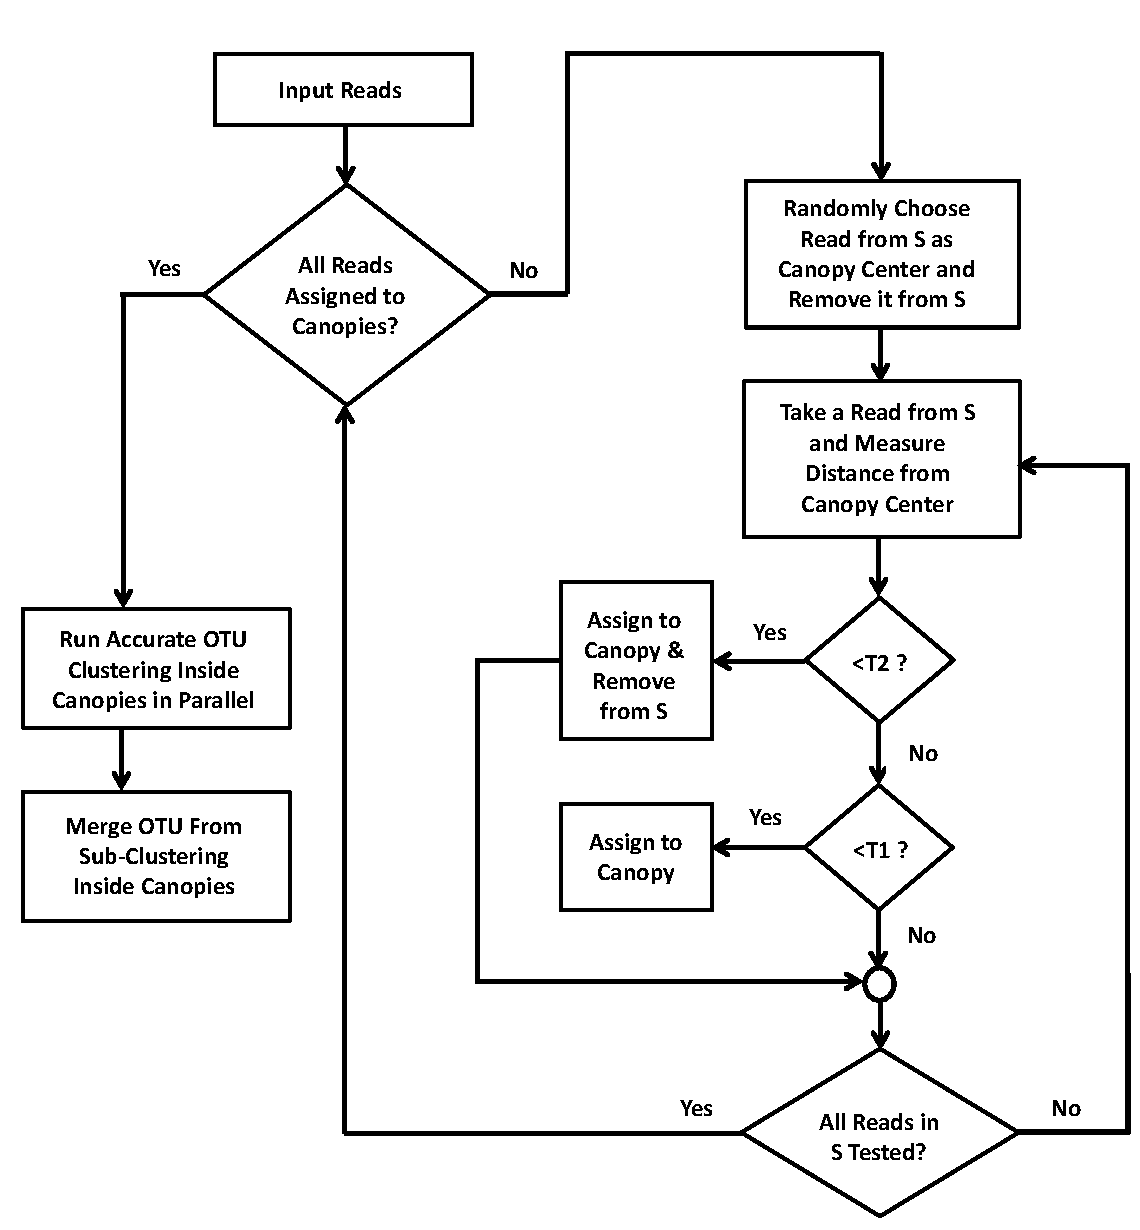
\includegraphics[width=\linewidth,height=10cm]{flowchart.pdf}	
	\caption{Workflow of Canopy Clustering for Large Scale Metagenome Data}
	\label{fig:flowchart}
\end{figure}

\subsection{Canopy Clustering}
Canopy Clustering\cite{MARCanopy} is an efficient 
approximate 
clustering algorithm often used as pre-processing step for other 
accurate and expensive clustering methods. It
is intended to speed up the 
clustering operations for 
large data sets by reducing number of pairwise distance calculations, where standard clustering algorithms may be 
impractical due to  run time and memory requirements. 

Canopy clustering uses two distance 
thresholds, (\romannum{1}) \textit{soft} threshold, $T1$ and (\romannum{2}) \textit{tight} threshold, $T2$. If a data instance 
$p_1$ is within the 
soft distance threshold $T1$ with centroid $C_a$ then $p_1$ will reside in same canopy as $C_a$. However,  $p_1$ may belong to other 
canopies assuming that it has only met soft threshold and it's 
best match is yet to be found. Thus one data point may belong to multiple canopies. However, 
if data point $p_1$ is within the tight distance threshold $T2$ with centroid $C_a$ then canopy clustering assigns $p_1$ to the  canopy with centroid $C_a$ 
and stops 
assigning $p_1$ to any other canopy. Initially, canopy centroids are selected 
randomly until all data points are
assigned to at least one canopy. 

\subsection{Locality Sensitive Hashing}
Canopies are intended to reduce the total pairwise distance calculations. As such, canopy clustering 
should be efficient, which requires a fast and approximate distance measure. Locality Sensitive Hashing (LSH)\cite{MARLshRef2} provides a solution for the approximate or exact near neighbors search problem. We construct the family of LSH functions with bit sampling\cite{indyk1998approximate}. Given an input vector $v$ and a random hyperplane defined by $r$; hash function $h(v)=\{0,1\}$ based on $sgn(v\cdot{r})=\pm{1}$ that indicates on which side of the hyperplane $v$ lies. For any $i^{th}$ bit, $h_i$ and for any two data instances $x,y$, 
the probability that $x$ and $y$ \emph{agree} on the $i^{th}$ positions of their respective $d$-length binary vector is

\begin{equation}
P[h_i(x)=h_i(y)]=1-\frac{f(x,y)}{d} 
\end{equation}

where $f(x,y)$ is the hamming distance and $d$ is the number of bits. The random projection and hamming distance calculation is computationally efficient making it suitable for fast partitioning of large volume of sequence reads. 

\subsection{Sub-Clustering Inside Canopies}
\label{sub-cluster}
Each of the canopy-based 
partitions are 
further clustered in parallel and independendtly 
with  expensive (but accurate)  clustering methods. We use UCLUST\cite{MARuclust}, SUMACLUST\cite{MARSumaclust} or 
SWARM\cite{MARSwarm2}  as accurate and 
expensive sub-clustering methods. 

\subsection{Merging Results from Canopies}
Each cluster (OTU) is represented by the Longest Common Subsequence of all member sequences. The final step of 
our proposed framework is to merge the 
OTU representations generated by the 
canopies. According to Canopy cluster algorithm a single data point may
belong to multiple canopies as long as the soft threshold is met. As a result 
similar OTU representations may appear from multiple canopies. To eliminate redundancy we run UCLUST on the 
OTU representations.

For notation purposes, 
the Canopy clustering (CC)  approach 
integrated with UCLUST, SUMACLUST and SWARM 
is denoted by CC$_{UCLUST}$, CC$_{SUMACLUST}$ and CC$_{SWARM}$, respectively. % where the term CC stands for Canopy Clustering. 

\section{Experimental Results}
\label{sec:Experimental}
\subsection{Dataset Description}
To evaluate the performance of our proposed approach we use previously 
published synthetic and real world 16S, 18S and metagenome sequence benchmarks. Key statistics 
regarding these datasets are presented in Table \ref{table:finaltabledataset}. 

\begin{table}[htb] 
	%\centering 
	\caption{\textbf{Dataset Statistics}}
	\label{table:finaltabledataset}
	\resizebox{\columnwidth}{!}{%
		\begin{tabular}{|l| c c c c|} 
			\hline
			\multirow{2}{*}{{\bf{Datasets}}} & \multirow{2}{*}{{\bf{Type}}} & {\bf{\# of}} & {\bf{\# of}}  & \multirow{2}{*}{\bf{Platform}}\\
			& & \bf{Reads} & \bf{Samples} & \\
			\hline
			{Bokulich$_2$} \cite{MARmockDatasetRef} & M & 6,938,836 & 4 & H\\
			{Bokulich$_3$} \cite{MARmockDatasetRef} & M & 3,594,237 & 4 & H\\
			{Bokulich$_6$} \cite{MARmockDatasetRef} & M & 250,903 & 1 & H\\
			{Canadian Soil} \cite{MARcanadianSoil} & R & 2,966,053 & 13 & H\\
			{Body Sites} \cite{MARbodySites} & R & 886,630 & 602 & G\\
			{Global Soil} \cite{MARglobalSoil} & R & 9,252,764 & 57 & H\\
			{Liver Cirrhosis} \cite{qin2014alterations} & R & 6,117,828,130 & 232 & H\\ 
			\hline
		\end{tabular}
	}
	\begin{tablenotes}
		\item Table shows information about dataset used in this study. M, R, H and G represent Mock, Real World, HiSeq and GS-FLX, respectively.		
	\end{tablenotes}
\end{table}	

\begin{table}[htb] 
	%\centering 
	\caption{\textbf{Parameter Settings}}
	\label{table:parameters}
	\resizebox{\columnwidth}{!}{%
		\begin{tabular}{|l| c c c c c|} 
			\hline
			Datasets & Total \# of & \# of Reads in &  & Parameters & \\
			\cline{4-6}			
			& Reads & Sampled Data & $d$ & $T1$ & $T2$ \\
			\hline
			{Bokulich$_2$} & 6,938,836 & 693,884 & 47 & 0.48 & 0.36\\
			{Bokulich$_3$} & 3,594,237 & 359,428  & 31 & 0.43 & 0.34\\
			{Bokulich$_6$} & 250,903 & 25,090 & 17 & 0.37 & 0.21\\
			{Canadian Soil} & 2,966,053 & 296,605 & 29 & 0.46 & 0.37\\
			{Body Sites} & 886,630 & 88,663 & 22 & 0.39 & 0.22\\
			{Global Soil} & 9,252,764 & 925,276 & 59 & 0.49 & 0.38\\
			{Liver Cirrhosis} & 3,000,000 & 300,000 & 48 & 0.42 & 0.35\\
			{Liver Cirrhosis} & 30,000,000 & 3,000,000 & 67 & 0.51 & 0.39\\ 
			\hline
		\end{tabular}
	}
\end{table}	 

\begin{table*}
	\centering
	\caption{\textbf{Runtime Comparison (in minutes)}} 
	\label{table:Runtime}
	\scalebox{0.62}{
		\begin{tabular}{|c c c|c c c|c c c|c c c|} 
			
			\hline
			
			\multicolumn{3}{|c|}{\textbf{Datasets}} & \multicolumn{9}{c|}{\textbf{Methods}}\\
			%\cline{3-9}
			
			\hline
			
			\multirow{1}{*}{Type} & \multirow{1}{*}{Title} & \multirow{1}{*}{\# of Reads} & \multirow{1}{*}{UCLUST} & \multirow{1}{*}{CC$_{UCLUST}$} & \multirow{1}{*}{Speed Up} & \multirow{1}{*}{SUMACLUST} & \multirow{1}{*}{CC$_{SUMACLUST}$} & \multirow{1}{*}{Speed Up} & \multirow{1}{*}{SWARM} & \multirow{1}{*}{CC$_{SWARM}$} & \multirow{1}{*}{Speed Up}\\
			
			\hline
			
			\multirow{3}{*}{\textit{Synthetic}} & Bokulich$_2$ & 6,938,836 & 12.71 & \textbf{3.08} & \textbf{4.13x} & 114.53 & \textbf{13.89} & \textbf{8.24x} & 128.12 & \textbf{17.24} & \textbf{7.43x}\\ 
			
			& Bokulich$_3$ & 3,594,237 & 10.43 & \textbf{3.61} & \textbf{2.89x} & 27.73 & \textbf{5.11} & \textbf{5.43x} & 18.37 & \textbf{3.39} & \textbf{5.41x}\\ 
			
			& Bokulich$_6$ & 250,903 & 4.47 &  \textbf{2.09} & \textbf{2.14x} & 5.61 & \textbf{2.07} & \textbf{2.71x} & 4.17 & \textbf{1.29} & \textbf{3.21x}\\ 
			
			\hline
			
			\multirow{3}{*}{\textit{Real World}} & Body Sites & 886,630 & 9.46 & \textbf{3.03} & \textbf{3.12x} & 18.42 & \textbf{6.02} & \textbf{3.06x} & 16.37  & \textbf{5.83} & \textbf{2.81x}\\
			
			& Canadian Soil & 2,966,053 & 13.65 & \textbf{4.17} & \textbf{3.27x} & 363.96 & \textbf{56.61} & \textbf{6.43x} & 117.53 & \textbf{20.84} & \textbf{5.64x}\\
			
			& Global Soil & 9,252,764 & 108.21 &  \textbf{18.75} & \textbf{5.77x} & 510.92 & \textbf{45.37} & \textbf{11.26x} & 289.51 &  \textbf{34.84} & \textbf{8.31x}\\
			
			& Liver Cirrhosis Metagenome & 3,000,000 & 14.57 &  \textbf{4.03} & \textbf{3.61x} & 46.62 & \textbf{9.02} & \textbf{5.17x} & 41.37 &  \textbf{8.75} & \textbf{4.73x}\\
			
			& Liver Cirrhosis Metagenome & 30,000,000 & 22.41h &  \textbf{1.84h} & \textbf{12.19x} & 46.62h & \textbf{2.21h} & \textbf{21.09x} & 37.43h &  \textbf{2.01h} & \textbf{18.61x}\\		
			
			\hline 
			
		\end{tabular}
	}
\end{table*} 

\subsubsection{Synthetic Datasets:}
The synthetic datasets are from Bokulich et al.\cite{MARmockDatasetRef} and 
available at QIIME database\footnote{http://qiime.org/home\_static/dataFiles.html} under their respective ID's. Since, these are simulated datasets the taxonomic profile of microbial organisms within them are known. We have used three well known simulated datasets Bokulich$_2$, Bokulich$_3$ and Bokulich$_6$. Bokulich$_2$, a simulated 16S rRNA gene microbial community dataset, was prepared using the Illumina TruSeq v2 paired--end library preparation kit. It contains 19 taxonomic families, 19 genera, 22 species and 22 strains in total. Bokulich$_3$ is similar to Bokulich$_2$ except that it was prepared with the TruSeq v1 paired-end library kit at Illumina Cambridge. Bokulich$_6$ is 16S rRNA dataset, sequenced at Washington University School of Medicine and contains evenly distributed microbial communities. This dataset contains 13 taxonomic families, 23 genera, 44 species and 48 strains in total.

\subsubsection{Real World Datasets}
\textbf{Canadian Soil:}
The Canadian Soil dataset\footnote{http://www.cm2bl.org/} contains genomic data of soil samples collected from across Canada spanning multiple biomes and ecozones.

\textbf{Body Sites:}
This dataset contains bacterial communities from up to 27 different body sites in healthy adults. A collection of 602 samples acquired from different body sites of human subjects are provided with meta-data.

\textbf{Global Soil:}
The global soil data was taken from Ramirez et al.\cite{MARglobalSoil} which is a study of the below-ground diversity in New York City's Central Park.

\textbf{Liver Cirrhosis:}
The Liver Cirrhosis dataset was taken from the study by Qin et al.\cite{qin2014alterations}. This is 
a whole gut microbiome wide association study of stool samples from 98 liver cirrhosis patients and 83 
healthy controls. Because of the high volume of sequence reads in this dataset, we used two random samples of 3 million and 30 million sequence reads from the original dataset.  

\subsection{Evaluation Metrics}
We evaluate the performance of our developed clustering approach using 
the following commonly used metrics that are used 
for the assessment of (i) outputs from clustering algorithms, (ii) biodiversity
within metagenome samples and (iii) computational run time. 

\subsubsection{Faith’s Phylogenetic Diversity Metric (PD)}
Faith’s phylogenetic diversity\cite{MARfaith1992conservation} combines all 
the branch lengths of phylogenetic tree as a measure of diversity. If a new 
OTU is found and it is closely related to another OTU in the sample, it will contribute to 
a small increase to the PD score. However, if a new OTU from different lineage is found then it will contribute to a large increase in the PD score.

\subsubsection{Shannon Entropy}
Shannon-Wiener diversity index is defined as:

\begin{equation}
H={-} \sum_{i=1}^{s} \left( p_i\log_2p_i \right)
\end{equation}

where s is the number of OTUs and $p_i$ is the proportion of the community represented by OTU $i$. The Shannon index increases as both the richness and evenness of the community increase.

\subsubsection{Simpson's Index}
Simpson’s index is defined as ${1-dominance}$ or

\begin{equation}
1 - \sum p_i^2
\end{equation}

where where $p_i$ is the proportion of the community represented by OTU $i$. Simpsonʼs index is based on the probability that any two individuals drawn at random from an infinitely large community belong to the same species.


\subsubsection{F-Score}
In case of synthetic datasets, expected taxonomic composition is known (\emph{ground truth}). False-positive (FP) 
refers to the number of taxonomy that was found in 
observed but not expected, false-negative (FN) refers to the number of taxonomy that exists in expected but not observed, and true-positive (TP) refers to the number of taxonomy exists in both observed and expected. The following definitions were used:

\begin{equation}
precision = \frac{TP}{(TP + FP)}
\end{equation}

\begin{equation}
recall = \frac{TP}{(TP + FN)}
\end{equation}

\begin{equation}
F Score = \frac{2 \times precision \times recall}{(precision + recall)}
\end{equation}

\subsubsection{Pearson Coefficient Correlation ($\rho$-value)}
After getting OTUs from a clustering method, we create a taxonomic profile at the Genus level. Pearson’s correlation coefficient was computed to measure the relatedness of taxonomic assignment between a pair of tools. Values range between -1 and 1, with -1 indicating a negative correlation, 0 indicating no correlation, and 1 indicating a positive correlation or strong relationship.

\subsection{Parameter Settings}
For kmers, the value of parameter $k$ was set to 4. The parameters for bit length of LSH ($d$), 
canopy's soft ($T1$) and 
hard ($T2$) thresholds were set by performing a grid search and validation. For validation purposes, 10\%  of the 
data was randomly sampled. First, the parameter for LSH 
bit length $d$ was estimated by fixing 
the soft ($T1$) and tight ($T2$) thresholds 
to 0.6 and 0.4, respectively.  $d$ was found to be proportional to the 
size of the input dataset. 
%
Once bit length for 
LSH  ($d$) was estimated we tuned values for $T1$ and $T2$ by decreasing $T2$ from 0.4 (\emph{relaxed}) to 0.1 (\emph{strict}) in steps of 0.01 and varying 
$T1$ from 0.6 to 0.1 in steps of 0.01. The parameters obtained on the 
validation sets for different benchmarks are 
shown in Table \ref{table:parameters}.

\subsection{Hardware and Software for Experiments}
We performed all the experiments on computers with Intel $5^{th}$ 
generation Core i7, 2.70 GHz 64bit processor with 8 core CPUs and 
12 GB memory. Sequence identity threshold for  
sub-clustering methods were set to default 97\%. For implementation we 
used Python 2.7.12 and QIIME\cite{MARQiime} version 1.9.0 (for diversity estimation).  Taxonomy for reported OTUs was assigned 
using the RDP Classifier\cite{MARRdp} against the 97\% representative databases for Greengenes\cite{MARGreen1} and Silva\cite{MARSilva}. We
used the PyNast\footnote{http://biocore.github.io/pynast/} open source sequence aligner
for aligning clustered output. 

\section{Result}
\label{sec:Results}
\subsection{Runtime Comparison} Table \ref{table:Runtime} shows the run time in minutes for 
UCLUST, SUMACLUST, SWARM and their respective versions with our proposed Canopy clustering pipeline. For the 30M sequence dataset, 
CC outperforms UCLUST, SUMACLUST and SWARM by 12.19, 21.09 and 18.61 times, respectively. For the Global Soil dataset 
CC outperforms UCLUST, SUMACLUST and SWARM by 5.77, 11.26 and 8.31 times, 
respectively. The highest gains in run time were found for the 
larger datasets demonstrating that 
CC scales well with large scale data. 

\subsection{Effect of Varying Number of Processors}
Figures \ref{fig:bokulich_2}-\ref{fig:global_soil} show the 
runtime of CC$_{UCLUST}$, CC$_{SUMACLUST}$ and CC$_{SWARM}$ on the 
two large 
benchmarks studied here. We observe that 
increasing number of processors reduces the 
total run time. Significant reductions in run time were 
observed for CC$_{SUMACLUST}$ and CC$_{SWARM}$ as 
compared to CC$_{UCLUST}$.  

\begin{figure}[t]	
	\begin{minipage}[t]{0.5\linewidth}
		\subfloat[]{
			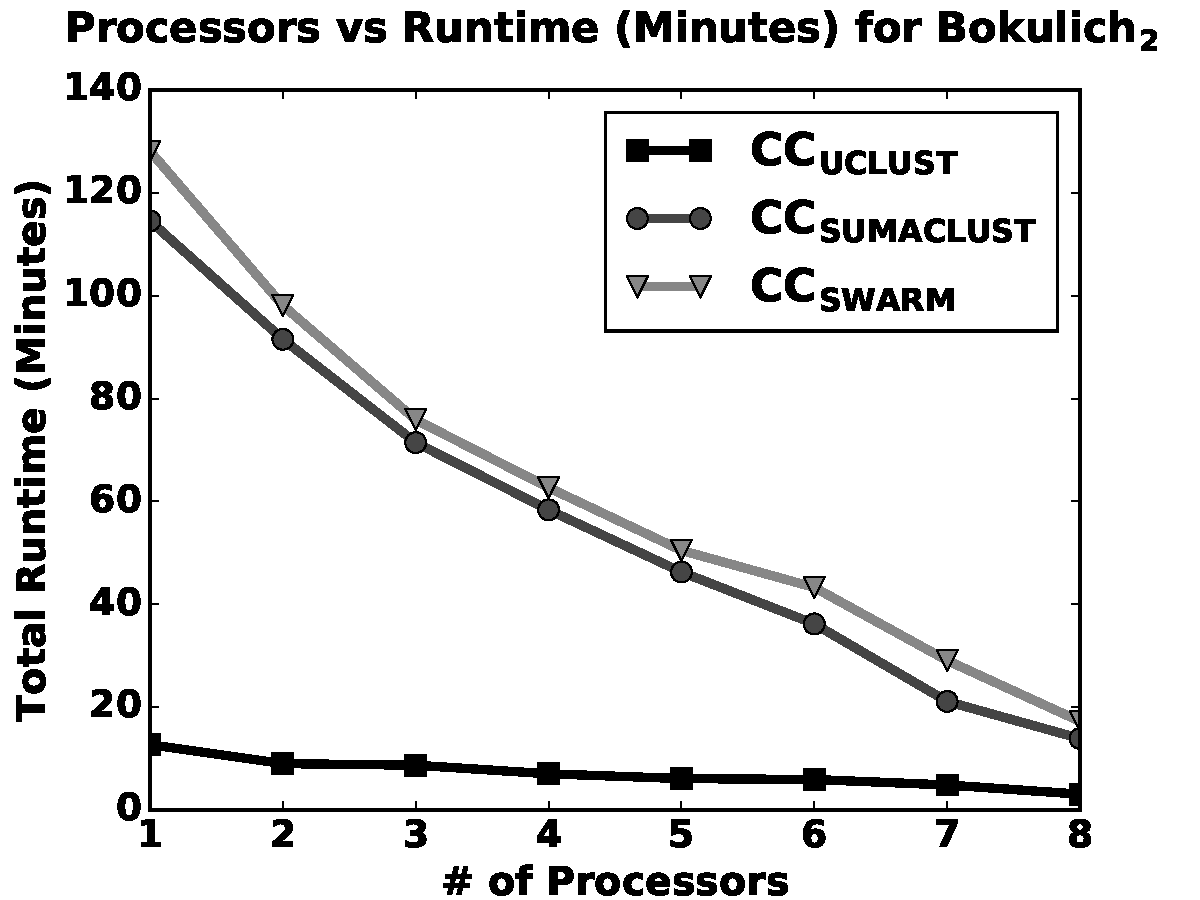
\includegraphics[width=\linewidth]{bokulich_2.pdf}
			\label{fig:bokulich_2}}
	\end{minipage}%
	\hfill%
	\begin{minipage}[t]{0.5\linewidth}
		\subfloat[]{
			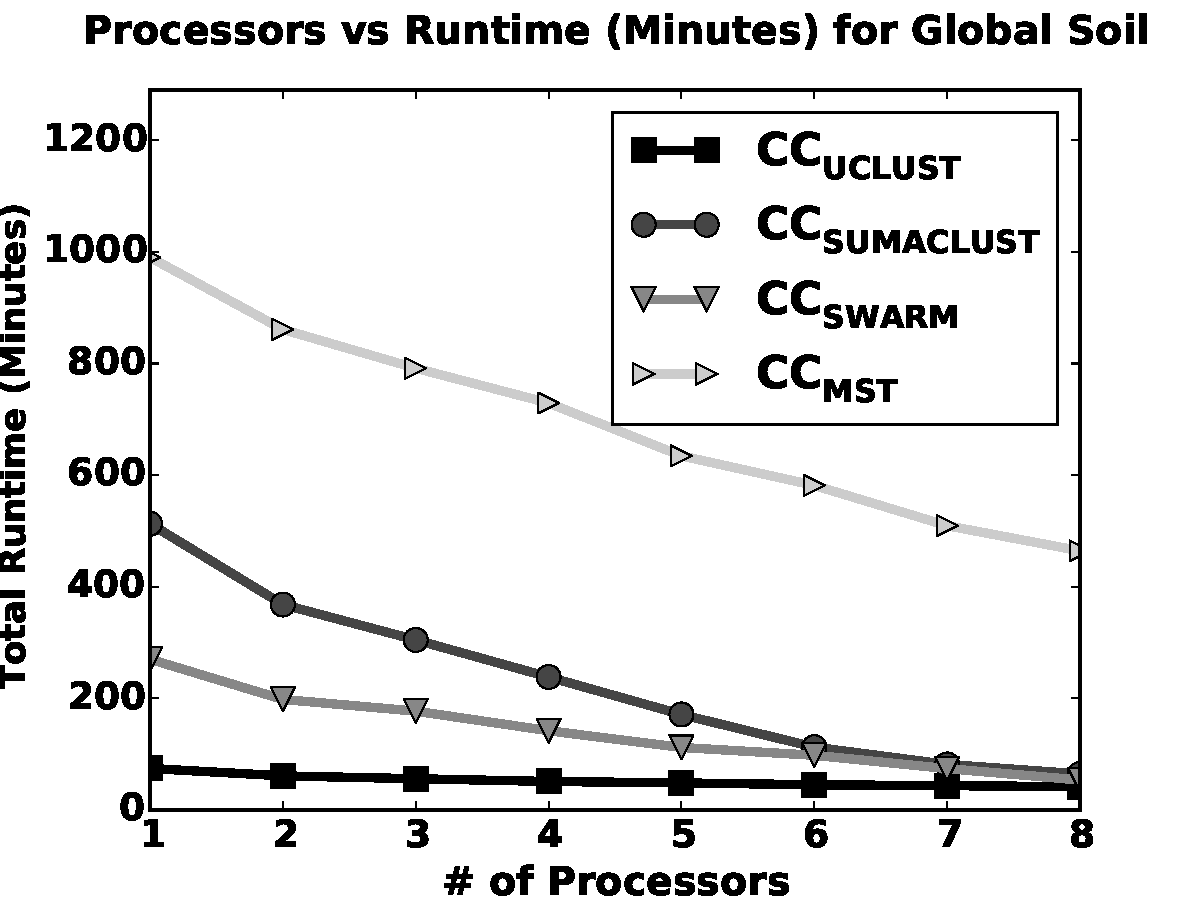
\includegraphics[width=\linewidth]{global_soil.pdf}
			\label{fig:global_soil}}
	\end{minipage}	
	\caption{Effect of number of processors on Runtime of CC$_{UCLUST}$, CC$_{SUMACLUST}$ and CC$_{SWARM}$ for 30M sampled dataset and Global Soil dataset, two of the largest datasets used in this study.}
\end{figure}

\begin{table*}[t]
	\centering 
	\caption{\textbf{Performance Comparison [$F$-Score and Pearson Correlation Coefficient ($\rho$)]}} 
	\label{table:performanceTable}
	
	\scalebox{0.66}{
		
		\begin{tabular}{|l|c c c c| c c c c c|}
			
			\hline
			
			\textbf{Methods} & \textbf{Comparison Metric} & \multicolumn{8}{c|}{\textbf{Datasets}}\\
			
			\cline{3-10}
			
			& & \multicolumn{3}{c|}{\textit{Synthetic}} & \multicolumn{5}{c|}{\textit{Real World}}\\ 
			
			\cline{3-10}
			
			%&  & Bokulich$_2$ & Bokulich$_3$ & Bokulich$_6$ & Body Sites & Canadian Soil & Global Soil\\
			
			&  &  &  & & & & & Liver Cirrhosis & Liver Cirrhosis\\
			
			& & Bokulich$_2$ & Bokulich$_3$ & Bokulich$_6$ & Body Sites & Canadian Soil & Global Soil & Metagenome & Metagenome\\
			
			& & & & & & & & (Sampled 3M) & (Sampled 30M)\\
			
			\hline
			
			\multirow{1}{*}{UCLUST} & $F$-Measure & 0.39 & 0.40 & 0.51 & $N/A$ & $N/A$ & $N/A$ & $N/A$ & $N/A$\\
			
			\hdashline
			
			\multirow{2}{*}{CC$_{UCLUST}$} & $F$-Measure & \textbf{0.39} & \textbf{0.41} & \textbf{0.52} & $N/A$ & $N/A$ & $N/A$ & $N/A$ & $N/A$\\
			& ($\rho$) with Respect to UCLUST & \textbf{0.9807} & \textbf{0.9753} & \textbf{0.9831} & \textbf{0.9682} & \textbf{0.8419} & \textbf{0.9824} & \textbf{0.9216} & \textbf{0.9072}\\
			
			\hline 
			
			\multirow{1}{*}{SUMACLUST} & $F$-Measure & 0.40 & 0.41 & 0.51 & $N/A$ & $N/A$ & $N/A$ & $N/A$ & $N/A$\\
			
			\hdashline
			
			\multirow{2}{*}{CC$_{SUMACLUST}$} & $F$-Measure & \textbf{0.41} & \textbf{0.42} & \textbf{0.51} & $N/A$ & $N/A$ & $N/A$ & $N/A$ & $N/A$\\
			& ($\rho$) with Respect to SUMACLUST & \textbf{0.9709} & \textbf{0.9813} & \textbf{0.9538} & \textbf{0.9518} & \textbf{0.7643} & \textbf{0.8714} & \textbf{0.9281} & \textbf{0.8614}\\ 
			
			\hline
			
			\multirow{1}{*}{SWARM} & $F$-Measure & 0.46 & 0.48 & 0.55 & $N/A$ & $N/A$ & $N/A$ & $N/A$ & $N/A$\\
			
			\hdashline
			
			\multirow{2}{*}{CC$_{SWARM}$} & $F$-Measure & \textbf{0.46} & \textbf{0.49} & \textbf{0.56} & $N/A$ & $N/A$ & $N/A$ & $N/A$ & $N/A$\\
			& ($\rho$) with Respect to SWARM & \textbf{0.9817} & \textbf{0.97861} & \textbf{0.9251} & \textbf{0.9648} & \textbf{0.7581} & \textbf{0.9143} & \textbf{0.9263} & \textbf{0.8533}\\
			
			\hline
			
		\end{tabular}
	}
	\small
	\begin{tablenotes}
		\item Table shows values of $F$-scores and Pearson Correlation Coefficient ($\rho$-value) of UCLUST, SUMACLUST, SWARM and their respective versions with Canopy clustering. $F$-measures is only available for synthetic datasets. $\rho$-value was calculated based on the taxonomy profiles at Genus level. Higher F-scores and $\rho$ values are represented with bold letters.         
	\end{tablenotes}
	
\end{table*}

\begin{table*}[t]
	\centering 
	\caption{\textbf{Biodiversity Comparison [Faith’s phylogenetic diversity metric (PD), Shannon and Simpson]}} 
	\label{table:bioDiversityTable}
	
	\scalebox{0.68}{
		
		\begin{tabular}{|c|c c c c| c c c c|}
			
			\hline
			
			\textbf{Methods} & \textbf{Comparison Metric} & \multicolumn{7}{c|}{\textbf{Datasets}}\\
			
			\cline{3-9}
			
			& & \multicolumn{3}{c|}{\textit{Synthetic}} & \multicolumn{4}{c|}{\textit{Real World}}\\ 
			
			\cline{3-9}
			
			&  &  &  & & & & & Liver Cirrhosis\\
			
			& & Bokulich$_2$ & Bokulich$_3$ & Bokulich$_6$ & Body Sites & Canadian Soil & Global Soil & Metagenome\\
			
			& & & & & & & & (Sampled 3M)\\
			
			\hline
			
			\multirow{3}{*}{UCLUST} & PD Range & $\left[171.95-221.85\right]$ & $\left[186.90-212.84\right]$ & $\left[104.51-104.51\right]$ & $\left[1.46-46.79\right]$ & $\left[0.30-1352.73\right]$ & $\left[2.98-3.29\right]$ & $\left[3.14-51.47\right]$\\ 
			& Shannon Range & $\left[2.52-3.51\right]$ & $\left[2.43-3.54\right]$ & $\left[5.87-5.87\right]$ & $\left[0.29-7.67\right]$ & $\left[2.32-7.86\right]$ & $\left[1.84-8.30\right]$ & $\left[0.27-5.77\right]$\\
			& Simpson Range & $\left[0.55-0.75\right]$ & $\left[0.55-0.76\right]$ & $\left[0.96-0.96\right]$ & $\left[0.049-0.98\right]$ & $\left[0.80-0.99\right]$ & $\left[0.0-0.98\right]$ & $\left[0.02-0.97\right]$\\
			
			& & & & & & & & \\
			
			\multirow{3}{*}{CC$_{UCLUST}$} & PD Range & $\left[164.79-217.72\right]$ & $\left[169.41-198.36\right]$ & $\left[109.33-109.33\right]$ & $\left[2.37-47.13\right]$ & $\left[0.52-1419.31\right]$ & $\left[3.02-3.81\right]$ & $\left[4.61-53.29\right]$\\
			& Shannon Range & $\left[2.61-3.83\right]$ & $\left[2.92-3.91\right]$ & $\left[6.41-6.41\right]$ & $\left[0.93-7.13\right]$ & $\left[3.26-7.61\right]$ & $\left[3.72-7.38\right]$ & $\left[0.13-6.17\right]$\\
			& Simpson Range & $\left[0.64-0.87\right]$ & $\left[0.56-0.93\right]$ & $\left[0.96-0.96\right]$ & $\left[0.081-0.99\right]$ & $\left[0.84-0.99\right]$ & $\left[0.21-0.99\right]$ & $\left[0.09-0.98\right]$\\
			
			\hline
			
			\multirow{3}{*}{SUMACLUST} & PD Range & $\left[106.00-162.78\right]$ & $\left[142.85-174.19\right]$ & $\left[89.22-89.22\right]$ & $\left[0.93-39.47\right]$ & $\left[0.59-1279.29\right]$ & $\left[2.98-3.29\right]$ & $\left[0.28-49.61\right]$\\
			& Shannon Range & $\left[2.00-3.01\right]$ & $\left[2.19-3.28\right]$ & $\left[5.48-5.48\right]$ & $\left[0.16-7.43\right]$ & $\left[2.32-7.32\right]$ & $\left[1.00-7.89\right]$ & $\left[1.37-7.83\right]$\\
			& Simpson Range & $\left[0.52-0.73\right]$ & $\left[0.54-0.75\right]$ & $\left[0.95-0.95\right]$ & $\left[0.027-0.98\right]$ & $\left[0.80-0.99\right]$ & $\left[0.40-0.98\right]$ & $\left[0.19-0.91\right]$\\
			
			& & & & & & & & \\
			
			\multirow{3}{*}{CC$_{SUMACLUST}$} & PD Range & $\left[114.96-171.57\right]$ & $\left[147.85-187.91\right]$ & $\left[93.81-93.81\right]$ & $\left[0.86-41.63\right]$ & $\left[0.81-1292.34\right]$ & $\left[1.37-4.89\right]$ & $\left[0.18-51.35\right]$\\
			& Shannon Range & $\left[2.51-3.94\right]$ & $\left[2.96-4.11\right]$ & $\left[5.94-5.94\right]$ & $\left[1.21-7.13\right]$ & $\left[3.12-7.79\right]$ & $\left[2.17-7.25\right]$ & $\left[1.91-7.39\right]$\\
			& Simpson Range & $\left[0.68-0.79\right]$ & $\left[0.51-0.74\right]$ & $\left[0.96-0.96\right]$ & $\left[0.06-0.99\right]$ & $\left[0.88-0.99\right]$ & $\left[0.23-0.98\right]$ & $\left[0.27-0.88\right]$\\
			
			\hline
			
			\multirow{3}{*}{SWARM} & PD Range & $\left[18.37-24.73\right]$ & $\left[17.36-19.81\right]$ & $\left[30.84-30.84\right]$ & $\left[1.44-28.66\right]$ & $\left[0.54-706.57\right]$ & $\left[5.79-6.18\right]$ & $\left[2.06-39.71\right]$\\ 
			& Shannon Range & $\left[2.98-3.91\right]$ & $\left[2.01-3.04\right]$ & $\left[5.03-5.03\right]$ & $\left[0.28-7.63\right]$ & $\left[1.0-7.79\right]$ & $\left[1.66-7.81\right]$ & $\left[1.47-6.91\right]$\\
			& Simpson Range & $\left[0.70-0.82\right]$ & $\left[0.53-0.74\right]$ & $\left[0.95-0.95\right]$ & $\left[0.05-0.98\right]$ & $\left[0.50-0.99\right]$ & $\left[0.00-0.99\right]$ & $\left[0.18-0.89\right]$\\
			
			& & & & & & & & \\
			
			\multirow{3}{*}{CC$_{SWARM}$} & PD Range & $\left[19.18-26.87\right]$ & $\left[18.43-22.61\right]$ & $\left[31.48-31.48\right]$ & $\left[2.34-29.97\right]$ & $\left[1.37-748.71\right]$ & $\left[2.34-8.46\right]$ & $\left[ 3.18-40.73\right]$\\
			& Shannon Range & $\left[1.66-4.87\right]$ & $\left[1.19-4.13\right]$ & $\left[6.03-6.03\right]$ & $\left[0.89-7.13\right]$ & $\left[2.81-8.06\right]$ & $\left[2.81-7.87\right]$ & $\left[2.03-6.88\right]$\\
			& Simpson Range & $\left[0.66-0.88\right]$ & $\left[0.41-0.81\right]$ & $\left[0.91-0.91\right]$ & $\left[0.11-0.99\right]$ & $\left[0.74-0.99\right]$ & $\left[0.14-0.99\right]$ & $\left[0.07-0.86\right]$\\
			
			\hline
			
		\end{tabular}
	}
	\small
	\begin{tablenotes}
		\item Table shows ranges of values for Faith’s Phylogeny Diversity (PD), Shannon and Simpson coefficient over all samples in a dataset in the format $[minimum-maximum]$. Most of these datasets contain multiple samples and Alpha diversity metrics like PD, Shannon and Simpson values are generated for each of these samples separately. Biodiversity metric values changes significantly over samples e.g. diversity from hair samples and teeth cavity are supposedly different. So instead of mean values this Table represents $[minimum-maximum]$  ranges of values a sample can take. Similar ranges reflect similar diversity.      
	\end{tablenotes}
	
\end{table*}

\subsection{Clustering Correctness}
Table \ref{table:performanceTable} shows the performance of  UCLUST, SUMACLUST and SWARM  in comparison to CC clustering versions. Table 
\ref{table:performanceTable} compares F-scores and Pearson Correlation Coefficient ($\rho$). F-scores 
are only available for synthetic 
benchmarks since taxonomic profile for them is known. Correlation values were generated 
based on taxonomic profiles at the 
Genus level, after obtaining final cluster output. We observe 
that F-scores obtained from a clustering method and its corresponding Canopy clustering version are very similar and in some 
cases better. For Bokulich$_3$ benchmark we observed higher F-scores for all $CC$ based methods. Finally for Bokulich$_6$ benchmark, the 
F-scores of CC$_{UCLUST}$ and CC$_{SWARM}$ were improved comparing to UCLUST and SWARM, respectively.
%
For all benchmarks we observe strong correlations between taxonomic profiles at genus level.

\subsection{Biodiversity Estimation} Table \ref{table:bioDiversityTable} shows the Faith’s phylogenetic diversity metric (PD), Shannon and Simpson index after clustering
with different methods. These metrics are 
popular Alpha Diversity metrics that measure species diversity in sites or habitats at 
a local scale. These metric values are generated per sample basis. Table \ref{table:bioDiversityTable} shows ranges of metric values
in $[minimum-maximum]$ format  for the different 
methods with and without Canopy clustering. From Table  \ref{table:bioDiversityTable}, we observe 
that Canopy clustering based methods produce similar ranges of values as their naive counterparts.

\subsection{Sensitivity Analysis (Varying T1 and T2)}
Figure \ref{fig:bokulich_2_T1}-\ref{fig:bokulich_2_T2} shows the 
effect of varying $T1$ ($T2$ fixed at 0.34) and $T2$ ($T1$ fixed at 0.45) on F-scores for the Bokulich$_2$ dataset. Reducing $T1$ leads to
comparatively \textit{strict} soft-threshold which will reduce 
repetitions of instances in multiple canopies. For a fixed $T2$ this implies that 
lower $T1$ will yield better canopy assignment. From Figure \ref{fig:bokulich_2_T1} we see that 
when $T1$'s range is in 0.4 to 0.6 our proposed approach provides better 
F-Scores. On the other hand, increasing $T2$ leads to comparatively \textit{relaxed} tight-threshold for canopies. As a result instances will be prematurely assigned to canopies without waiting for best match. From Figure \ref{fig:bokulich_2_T2} we note that 
when $T2$  is in between 0.25 to 0.35, 
our proposed approach achieves better F-Scores. Lowering 
$T2$ may lead to higher run time since instances will continue to reappear 
until the $T2$ threshold is satisfied.                   

\begin{figure}[t]	
	\begin{minipage}[t]{0.5\linewidth}
		\subfloat[]{
			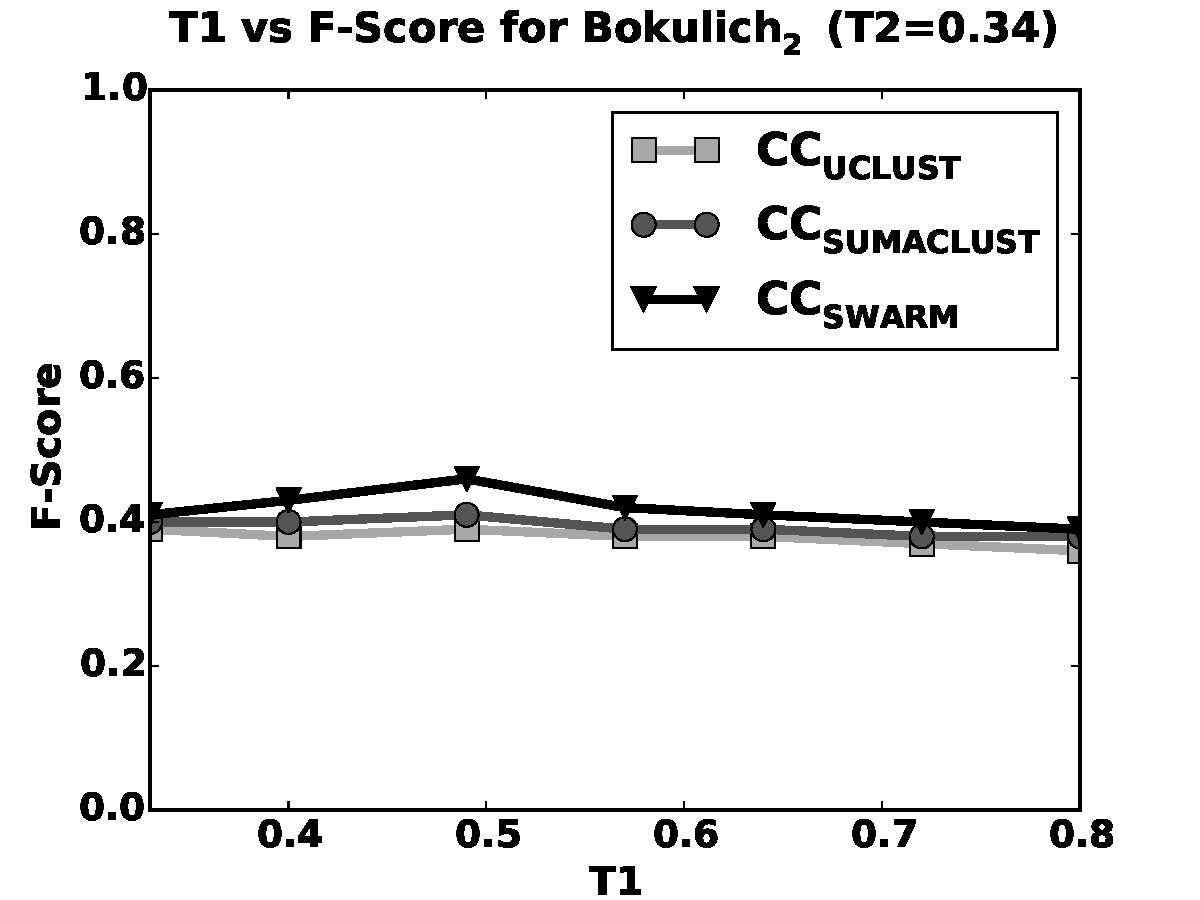
\includegraphics[width=\linewidth]{bokulich_2_T1.pdf}
			\label{fig:bokulich_2_T1}}
	\end{minipage}%
	\hfill%
	\begin{minipage}[t]{0.5\linewidth}
		\subfloat[]{
			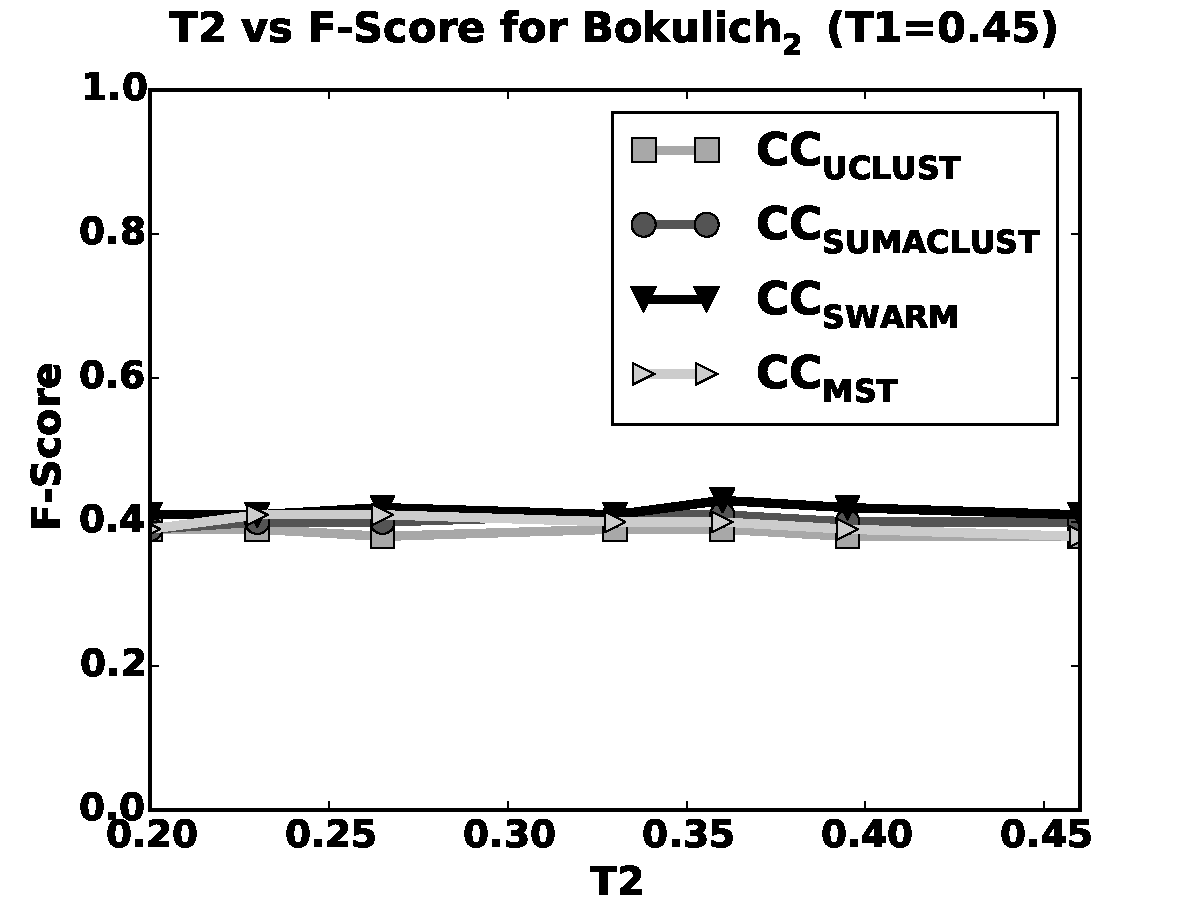
\includegraphics[width=\linewidth]{bokulich_2_T2.pdf}
			\label{fig:bokulich_2_T2}}
	\end{minipage}
	\caption{ \ref{fig:bokulich_2_T1} and \ref{fig:bokulich_2_T2} show effect of varying $T1$ and $T2$ on $F$-scores for the largest synthetic dataset Bokulich$_2$ }	
\end{figure}

\section{Conclusion}
\label{sec:Conclusion}
We developed a greedy clustering algorithm 
that scales to large metagenome sequence datasets. The strengths of our proposed approach is that it can be integrated as a pre-processing step
with state-of-the-art expensive but accurate clustering algorithms allowing them to
operate efficiently on real world datasets. 
%
Our approach 
achieves efficiency 
by  
partitioning the large number of sequence reads into 
groups (called canopies) using locality sensitive 
hashing.  This 
initial approximate assignment of sequence reads to 
canopies is then 
refined. We demonstrate that our 
approach provides similar outcome in terms of biodiversity metrics, ground truth and taxonomic correlation with corresponding expensive clustering methods.
%
We show significant reduction in run times in comparison to previously developed sequence 
clustering algorithms, especially on datasets with millions of sequence reads.


\bibliographystyle{plain}
\bibliography{myRef} 



\end{document} 